\documentclass[12pt,a4paper]{article}

\usepackage[utf8]{inputenc}

\usepackage[width=190mm,height=272mm,centering]{geometry}

% \usepackage{mathptmx}
\usepackage{palatino}

%\usepackage{chancery}
%\usepackage{antiqua}
%\usepackage{aboensis}
\usepackage{gfsartemisia-euler}
\usepackage[T1]{fontenc}

% \usepackage{fontspec}
% \setmainfont{QTChanceryType}

\usepackage{graphicx}
\usepackage[table]{xcolor}
\usepackage{tikz}
%\usetikzlibrary{decorations.text}
\usepackage[hidelinks]{hyperref}

\pagestyle{empty}

%\newcommand{\logo}{\makebox[56mm][c]{\rule{0mm}{66mm}\raisebox{12mm}{\includegraphics[width=48mm]{logo/aldc-4couleurs-3.pdf}}}}

%\pagecolor{yellow!5}

\usepackage{fontspec}
\usepackage{eurosym}

\begin{document}
\sffamily
\bfseries
%\color{yellow!20}
\parindent=0mm

%%%%%%%%%%%%%% FOND ET LOGOS

\unitlength=1mm
\begin{picture}(0,0)
%\put(-22,-150){\includegraphics[width=212mm]{images/lambris-chene-clair.png}}
%\put(-16,-200){\includegraphics[width=212mm]{images/lambris-chene-clair.png}}
\put(-11,-280){\includegraphics[width=212mm]{images/Fond-bois-tres-clair-small.jpg}}
%\put(15,-274){\includegraphics[width=140mm]{images/groupe.pdf}}
\put(15,-270){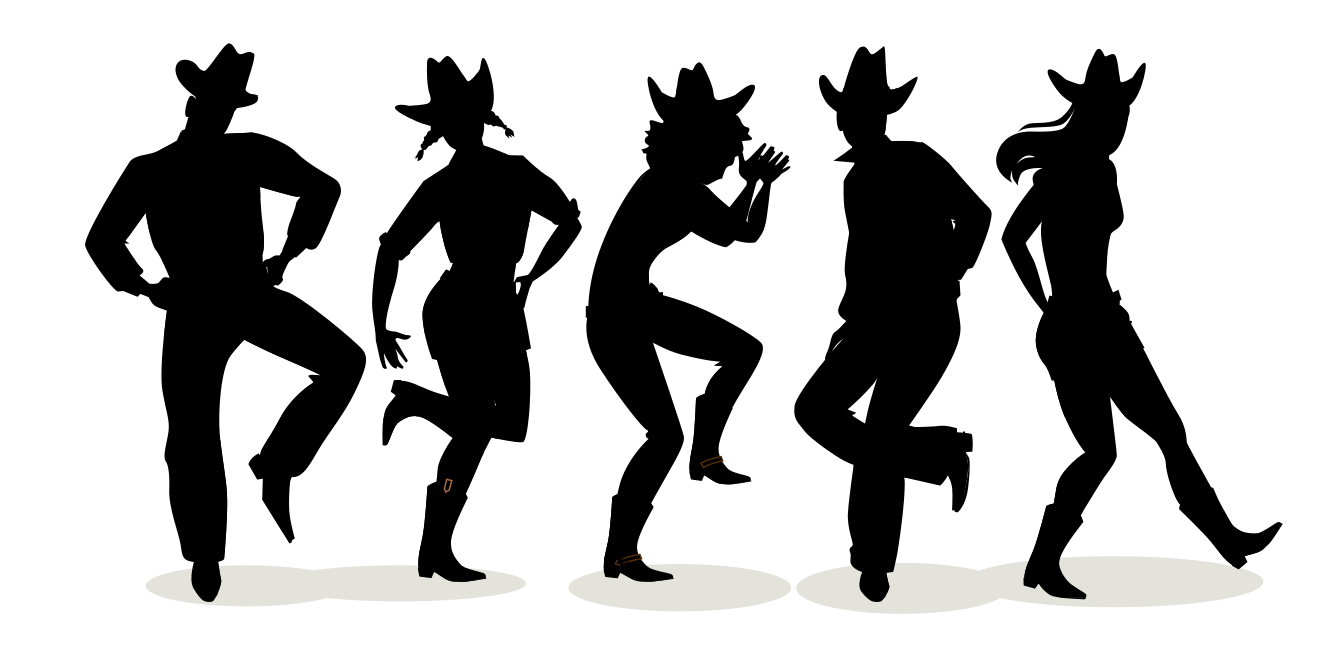
\includegraphics[width=170mm]{images/groupededanseenligne-ombre.png}}
%\put(-3,-274){\href{https://alevisdanse.github.io}{\includegraphics[width=40mm]{images/qr-code.pdf}}}
%\put(-3,-274){\includegraphics[width=100mm]{images/Exposants.png}}
%\put(20,-274){\includegraphics[width=80mm]{images/Vero'sBoutik.png}}
%\put(90,-210){\includegraphics[width=100mm]{images/Charlie-Gon.png}}
\put(145,-30){\href{https://alevisdanse.github.io}{\includegraphics[height=40mm]{static/images/logo-aldc-contour-noir.pdf}}}
\put(-5,-35){\href{https://country-rn10-13.webself.net/}{\includegraphics[height=50mm]{images/LOGO RN10 officiel-fi36141364x430.png}}}
\end{picture}


\vspace*{35mm}

\fontsize{64pt}{64pt}
\fontspec{QTOKCorral-Ext}
\selectfont

\begin{center}

  \begin{tabular}{p{0.6\textwidth}@{\hspace*{2mm}}r}
    Bière & 2,50 \euro \\

    Soda & 1,50 \euro \\

    Eau & 0,50 \euro \\

    Café/Thé & 1 \euro \\

    Crêpe sucre & 1 \euro \\

    Crêpe Nutella & 1,50 \euro \\

    Pâtisserie & 1 \euro \\

    Sandwich  & 3 \euro \\

    Formule \fontsize{40pt}{40pt}\selectfont(sandwich + \hspace*{20mm}\hfill pâtisserie + boisson) & 5 \euro \\
  \end{tabular}
\end{center}

\end{document}
